\chapter{Artificial Intelligence for Sagrada}

\section{Board Evaluation}

When crafting an AI agent for games, especially strategy-based ones like Sagrada, the ability to evaluate the 
game board accurately is paramount. This evaluation serves as the foundation upon which the agent makes its decisions, 
determining the quality of its moves and ultimately its success or failure. By evaluating the board, the AI agent can 
anticipate future developments and plan its moves accordingly. It can identify key objectives, assess potential risks, 
and devise multi-step strategies to achieve its goals.  Evaluating the board efficiently is crucial for ensuring that 
the AI agent can process information and make decisions under a given time limit. 

\subsection{Board Evaluation in Sagrada} \label{subsec:Board_Evaluation_In_Sagrada}

Evaluating players' boards is one of the functionalities of the Model component. The Score class is responsible for evaluating
the state of a given player including a board evaluation and the points for the unused favor tokens. Each Score object contains
the following components:
\begin{itemize}
    \item The number of penalty points received for each empty field
    \item The number of Private Objective Card points received by the player
    \item A vector of PuocPatternState objects each representing the state of a concrete Public Objective Card
    \item The final score of the player
\end{itemize}

\subsubsection{PuocPatternState}
PuocPatternState objects represent the state of a board from the perspective of a given Public Objective Card. These objects
are constructed by the Public Objective Cards during the board evaluation. They contain both rules-based information 
(currently earned points) and heuristic-based information (the heuristic state).

The heuristic-based pattern evaluation is divided into completable and uncompletable patterns. I simply count the uncompletable
patterns but for completable patterns, I remember the number of dice that are missing to match
the given pattern. This makes the evaluation of given patterns stronger because given agents can reward
placing dice that make closer patterns to completion. 

The performance of an evaluation function is critical for agents utilizing algorithms like Minimax, particularly in complex games 
such as Sagrada, where the branching factor is high. Certainly, there's often a trade-off between the accuracy and efficiency of an evaluation function. 
However, despite these occasional inaccuracies, the overall performance of the AI agent might still be satisfactory.
One of the inaccuracies occurs when evaluating Public Objective Cards that contain either a row or a column matching for unique dice colors or shades.
The reason behind this behavior is that each row/column is evaluated independently. However, the neighboring rows/columns have an impact on each other.


I will demonstrate this phenomenon in an example. Let's say one of the Public Objective Cards is the Row Shade Variety. This means we are trying
to place dice so each row contains dice with unique shades. The following figure shows an example state:


\begin{figure}[H]
    \caption{ Incorrect evaluation board position example}
    \centerline{\mbox{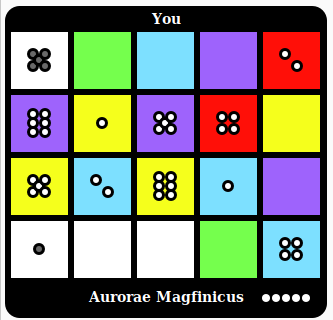
\includegraphics[width=100mm]{img/IncorrectBoardEvaluationExample.png}}}
    \label{fig:example}
\end{figure}


Please notice that the second row could be completed with a 2 or a 3, and the third row could be completed with a 3 or a 4. Since the first row
contains a red die with the value of 2 at the rightmost column, a die having a value of 2 cannot be placed to the neighboring fields so the only 
value left for completing the second row is 3. The same principle applies to the third row and the blue 4 die in the fourth row. This means that 
both rows can be completed only with a 3 which is not possible because of the rules of the game. However, the board evaluation processes the rows
independently, it will report that both of these rows can be finished at the same time. The reason behind not implementing it perfectly is connected
to performance. This phenomenon occurs rarely and avoiding it would require looking for a concrete placing of dice to each empty field. Approaching
to implement this feature was considered not worth the performance overhead.


\section{Branching Factor}

The concept of branching factor refers to the number of possible moves available to players at any given point in the game.
In the realm of AI algorithms, the branching factor stands as a key metric defining the number of possible actions or choices available to the agent at 
each decision point within a search tree. Understanding its importance is paramount, as it profoundly influences the computational complexity, efficiency, 
and effectiveness of various search-based algorithms. A higher branching factor exponentially increases the number of possible paths within the search tree, 
rapidly escalating the computational requirements of the algorithm. 

In search-based algorithms like minimax and MCTS, the branching factor profoundly impacts the efficiency of the search process. A lower branching factor 
typically leads to more efficient exploration of the search space, as the algorithm can delve deeper into the tree without sacrificing computational resources. 
Conversely, a higher branching factor necessitates shallower search depths or more aggressive pruning strategies to maintain acceptable performance levels.

The branching factor varies throughout the game, influenced by factors such as the stage of the game and the presence of 
different types of tool cards. Some tool cards provide players with straightforward actions, resulting in a consistent 
branching factor of one for each use. In contrast, other tool cards introduce variability in branching factor, as their effects 
may differ based on the current state of the game or player choices. For example, tool cards that allow players to relocate dice 
on a board can dramatically increase the branching factor by introducing a huge amount of possibilities.

Introducing two basic AI agents: the Random Agent, which chooses moves randomly, and the First Agent, selecting the first possible move at each decision point.
The following figure illustrates the branching factor of the Random and First Agents across the rounds of the game.


\begin{figure}[H]
    %\captionsetup{position=above}
    %\centering
    \caption{ Branching factor across the rounds for random agents}
    \centerline{\mbox{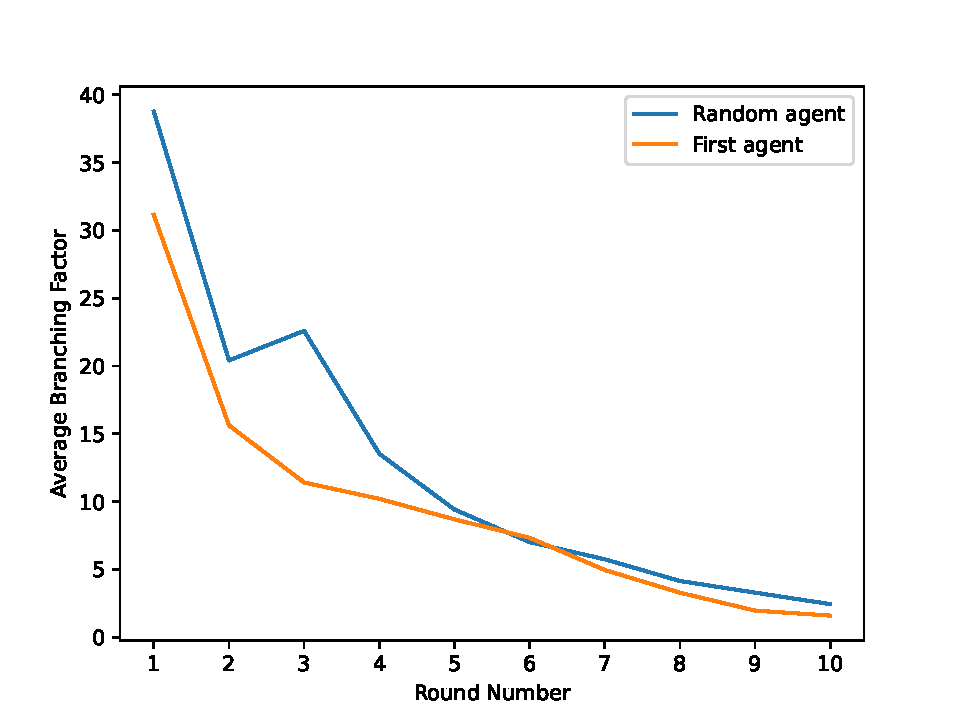
\includegraphics[width=150mm]{img/random_agents_branching_factor.pdf}}}
    \label{fig:example}
\end{figure}


\subsection{Smarter players} \label{subsec:smarter_player_branching_factor}
While the random agents provide a baseline understanding of the branching factor in the game, it's crucial to acknowledge that more strategic or skilled players 
will exhibit different branching factors. Smarter players tend to explore deeper and more selectively within the game tree, leading to a narrower but more focused 
set of potential moves. 


\section{Heuristic Filter} \label{sec:Heuristic_filter}

Heuristic filters play a crucial role in AI algorithms, particularly in scenarios where exhaustive search or perfect evaluation is impractical due to 
computational constraints. Heuristic filters help narrow down the search space by quickly discarding unpromising choices, allowing the AI algorithm to 
focus its computational resources on more promising alternatives. 

One common pitfall is inadvertently limiting future placement options by positioning dice in a way that conflicts with the game's color or shade restrictions. 
Recognizing this, a heuristic filter can be employed to identify and avoid such "bad moves", both in regular die-to-field placements and when utilizing Tool Cards.
When considering potential moves for placing a die on the board, the heuristic filter evaluates each option to determine if it would place a die adjacent to a field 
that shares the same color or shade restriction as the placed die. If such a placement would impede future options, it's flagged as undesirable and filtered out. 
By proactively avoiding these conflicting placements, the AI ensures that it maintains flexibility and maximizes its future placement opportunities.
Similarly, when utilizing Tool Cards, the heuristic filter examines the potential outcomes of each action to identify any placements that would create conflicts with 
existing dice on the board. Whether it's using a Tool Card to manipulate dice placements or draft additional dice, the AI applies the same logic to ensure that its 
moves align with its long-term strategic objectives.

Using this filtering method, all the possible moves are separated into "good moves" and "backup moves" that are used when there are no "good moves" to work with.

\section{Heuristic Sort} \label{sec:Heuristic_sort}

Heuristic sorting of moves plays a pivotal role in modern AI algorithms for board games, providing a strategic advantage by guiding the AI agent towards more promising moves of play. 
Furthermore, heuristic sorting facilitates the exploration of deeper and more complex game trees within a limited computational budget. In games with high branching factors, 
heuristic sorting allows AI agents to efficiently allocate their resources towards exploring the most promising branches of the game tree. Since the comparator is executed numerous times, 
its efficiency is critical to ensure the overall speed and responsiveness of the sorting algorithm.

We have already talked about filtering the least promising moves in the previous section. This section provides a deeper understanding of how the remaining moves are sorted.
Due to the time limit, we cannot use any heuristic-based sorting technique that would be connected to the Public Objective Card patterns. There is one component in the scoring
structure that is easy to use as the base of the sorting algorithm being the Private Objective Card's color.

The sorting algorithm decides between two moves according to the following criteria:
\begin{enumerate}
    \item If none of the moves is a DTFM, a random move is prioritized
    \item If one of the moves is a DTFM and the other one is not, the DTFM is prioritized. 
    \item If one of the dice matches the color of the Private Objective Card and the other does not, the die matching the Private Objective Card color is prioritized.
    \item If one move places a die to a field that has a restriction and the other one does not, the one placed to a field with a restriction is prioritized.
    \item Finally, the die with the higher value is prioritized.
\end{enumerate}